\documentclass[10pt]{article}
\usepackage[utf8]{inputenc}
\usepackage[T1]{fontenc}
\usepackage{amsmath}
\usepackage{amsfonts}
\usepackage{amssymb}
\usepackage[version=4]{mhchem}
\usepackage{stmaryrd}
\usepackage{graphicx}
\usepackage[export]{adjustbox}
\graphicspath{ {./images/} }

\title{Probability and Statistics \\
 Simulation }

\author{Giuliano Casale\\
Department of Computing, Imperial College London}
\date{}


%New command to display footnote whose markers will always be hidden
\let\svthefootnote\thefootnote
\newcommand\blfootnotetext[1]{%
  \let\thefootnote\relax\footnote{#1}%
  \addtocounter{footnote}{-1}%
  \let\thefootnote\svthefootnote%
}

%Overriding the \footnotetext command to hide the marker if its value is `0`
\let\svfootnotetext\footnotetext
\renewcommand\footnotetext[2][?]{%
  \if\relax#1\relax%
    \ifnum\value{footnote}=0\blfootnotetext{#2}\else\svfootnotetext{#2}\fi%
  \else%
    \if?#1\ifnum\value{footnote}=0\blfootnotetext{#2}\else\svfootnotetext{#2}\fi%
    \else\svfootnotetext[#1]{#2}\fi%
  \fi
}

\begin{document}
\maketitle
Based on slides by Tony Field.

\section*{Simulation}
Broadly, there are multiple classes of simulation:

\begin{itemize}
  \item Monte Carlo: aggregate the results of a series of "one shot" experiments using random numbers
  \item Discrete time: perform an $n$-step random state transitions, moving from one state to another in each (discrete) step.\\
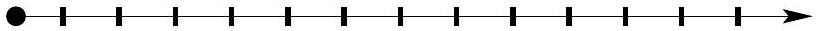
\includegraphics[max width=\textwidth, center]{2025_05_12_520db7cd238ba7b44f0fg-02(1)}
  \item Continuous time: System state is continuously evolved over time as a result of a prescribed dynamics.
  \item Discrete event: System state transitions are triggered by events occurring at discrete points in continuous time.\\
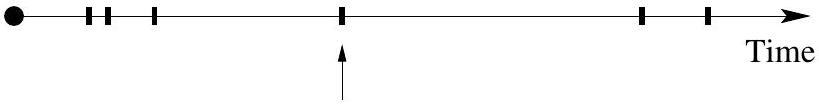
\includegraphics[max width=\textwidth, center]{2025_05_12_520db7cd238ba7b44f0fg-02}
\end{itemize}

An event

\section*{Example: Monte Carlo simulation}
\begin{itemize}
  \item Estimate $\pi$ by random sampling:\\
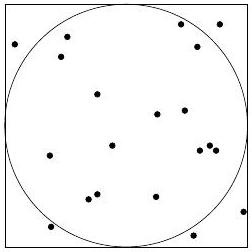
\includegraphics[max width=\textwidth, center]{2025_05_12_520db7cd238ba7b44f0fg-03}
  \item Assume the circle has radius $r$ so the square is $2 r \times 2 r$
  \item Pick $N$ random points inside the square, then:\\
$\frac{\text { No. samples in circle }}{\text { No. samples in square }} \approx \frac{\pi r^{2}}{(2 r)^{2}}=\frac{\pi}{4}$
\end{itemize}

\section*{Example: Discrete-Time Simulation}
\begin{itemize}
  \item What's the steady-state probability, $p_{i}$, of ending up on square $i$ at the end of a move in a game of Monopoly (39 possibilities)
  \item The game may be modelled as a DTMC\\

\includegraphics[max width=\textwidth, center]{2025_05_12_520db7cd238ba7b44f0fg-04}
  \item Start at GO, simulate $N$ moves, implementing the rules of the game. Then, $p_{i} \approx$ (no. times move ended on $i$ ) / $N$.
  \item There is no explicit notion of time here, although we could assume each move takes some fixed time, $T$, say.
\end{itemize}

\section*{Example: Continuous-Time Simulation}
\begin{itemize}
  \item Simulation dynamics is often described by physical laws\\
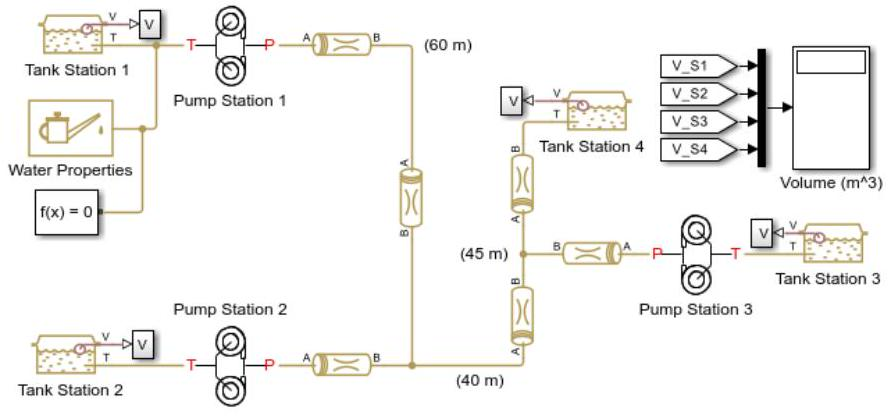
\includegraphics[max width=\textwidth, center]{2025_05_12_520db7cd238ba7b44f0fg-05}
  \item Simulate time using infinitesimal time steps ( $d t$ increments).
  \item Typically, a vector of state variables $\mathbf{x}(t)$ is evolved via ODEs $\frac{d}{d x} \mathbf{x}(t)=A \mathbf{x}(t)$, given an initial state $\mathbf{x}(0)=x_{0}$.
\end{itemize}

Image source: Mathworks

\section*{Discrete Event Simulation (DES)}
\begin{itemize}
  \item A (discrete-event) simulation is a program that generates a random sample path through a state transition system, where time delays are associated with each state
  \item There is a single global "clock" - a virtual time. Not to be confused with elapsed real time.
  \item State transitions are triggered by events which are ordered in time on a virtual timeline, an event "diary".
  \item DES involves invoking events in time order; if an event is invoked ("occurs", "fires", "is triggered", ...) at virtual time $t$ the clock is updated to $t$ and the code for the event:
  \item Updates the model state
  \item Schedules zero or more new future events on the time line
  \item Note that the state is unchanged between events
\end{itemize}

\section*{Discrete Event Simulation}
\begin{itemize}
  \item In practice, DES is based on a few core design principles:
  \item The virtual time is a floating-point number (call it now)
  \item The state is defined by a set of program variables, which are typically discrete (e.g. booleans, integers, ...) ${ }^{1}$
  \item The timeline is a priority queue of (Event, time) pairs, ordered by virtual time - essentially an event diary
  \item Events are implemented as objects, functions, procedures, methods, etc.
  \item A scheduler adds new (Event, time) pairs to the diary
  \item A descheduler similarly removes them from the diary
  \item Additional measurement variables and code need to be added in order to accumulate performance measures (otherwise there will be no output!)
\end{itemize}

\footnotetext{${ }^{1}$ A DES may include continuous state variables (e.g. doubles) but they can only change in discrete steps, e.g. a petrol pump from which petrol is drained instantaneously for the purposes of the model
}\section*{Evolving time}
\begin{center}
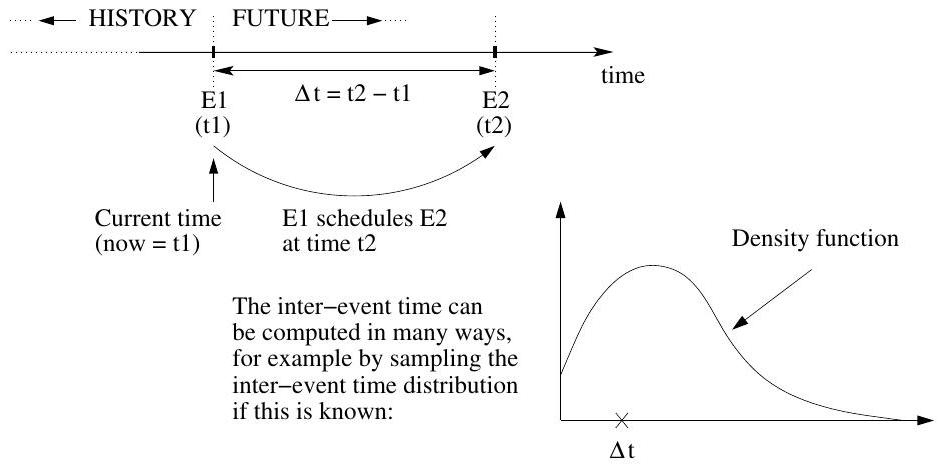
\includegraphics[max width=\textwidth]{2025_05_12_520db7cd238ba7b44f0fg-09}
\end{center}

\begin{itemize}
  \item The times between events are r.v.s with an associated distribution - inter-event times are samples from that distribution
  \item We need to be able to sample these distributions
\end{itemize}

\section*{Example: A Single-server FIFO Queue}
\begin{itemize}
  \item Consider a single-server queue with some specified inter-arrival time and service time distribution and a queue with finite capacity N (jobs in the buffer + job in service)\\
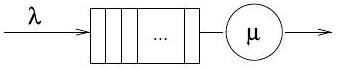
\includegraphics[max width=\textwidth, center]{2025_05_12_520db7cd238ba7b44f0fg-10}
  \item The simplest model identifies an integer state with each queue population ( $0,1,2 \ldots$ ):\\
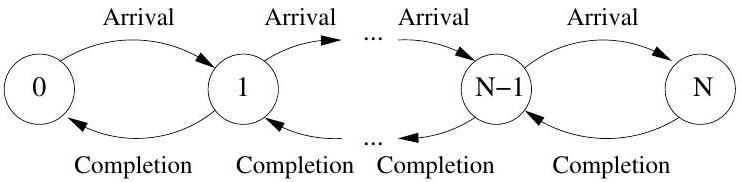
\includegraphics[max width=\textwidth, center]{2025_05_12_520db7cd238ba7b44f0fg-10(1)}
  \item We require two events (Arrival and Completion)
  \item The time line (priority queue) contains arrival and completion events that have yet to occur\\
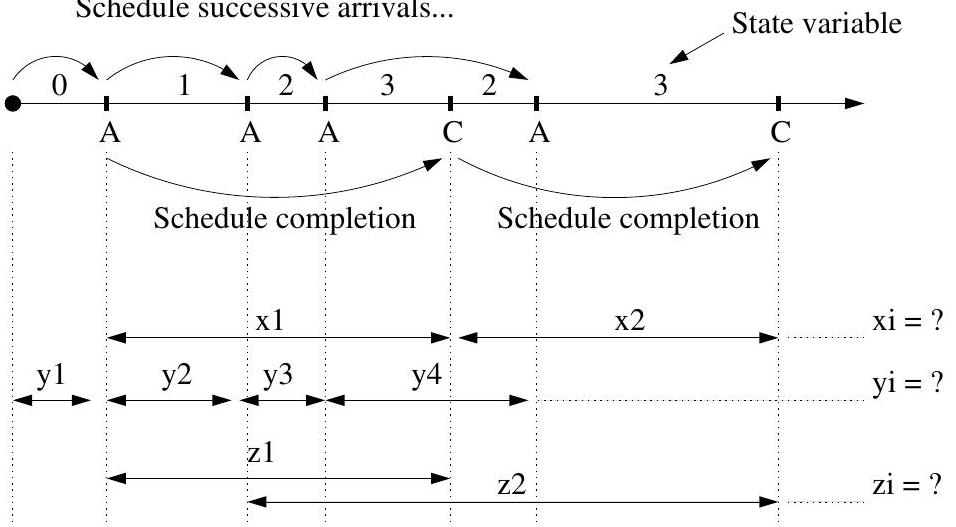
\includegraphics[max width=\textwidth, center]{2025_05_12_520db7cd238ba7b44f0fg-11}
  \item Model code sketch (Note: Code in these slides and coding exercises are not examinable.)
\end{itemize}

\begin{verbatim}
State variable (population):
    int n = 0
Arrival:
    n++
    if n < N
        t = sample from inter-arrival time distribution
        schedule a new arrival at time t from now
    if n == 1
        t' = sample from service time distribution
        schedule a new completion at time t' from now
\end{verbatim}

\section*{Continued...}
Completion:

\begin{verbatim}
n--
if n == N-1
    t = sample from inter-arrival time distribution
    schedule a new arrival at time t from now
if n > O
    t' = sample from service time distribution
    schedule a new completion at time t' from now
\end{verbatim}

\begin{itemize}
  \item We kick start it by scheduling the first arrival and terminate after a specified number of arrivals, or a given termination time
\end{itemize}

\section*{Designing a simulation model}
(1) Identify the entities in the system that have to be modelled\\
(2) Identify the model states (program state variables) - these specify where each entity is and what it is doing\\
(3) Identify the event types, recalling that each state transition is triggered by an event (note that some events may be parameterisable, e.g. "arrival at location a")\\
(9) For each event, specify i. how it changes the current state, ii. what new events need to be scheduled and what old events need to be cancelled (descheduled) when it fires\\
(9) Add code to accumulate measurements whilst the simulation executes\\
(- Add code to output results when the program terminates, e.g. after $T$ simulated time units, $N$ occurrences of a specified event, etc.

\section*{Output Analysis}
\section*{Terminating vs Non-terminating Simulation}
\begin{itemize}
  \item A non-terminating simulation, seeks to model a system at "equilibrium", a.k.a. "in steady state", where $p_{s}(t) \rightarrow p_{s}$ as $\rightarrow \infty$\\
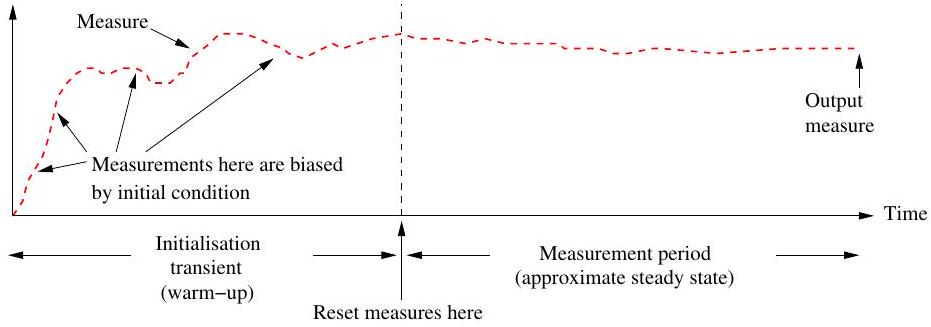
\includegraphics[max width=\textwidth, center]{2025_05_12_520db7cd238ba7b44f0fg-16}
\end{itemize}

\section*{Terminating vs Non-terminating Simulation}
\begin{itemize}
  \item A terminating simulation models a system over a specified period during which there is no notion of equilibrium, e.g.\\
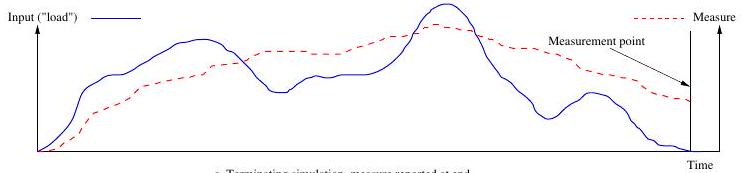
\includegraphics[max width=\textwidth, center]{2025_05_12_520db7cd238ba7b44f0fg-17}\\
a. Terminating simulation, measure reported at end
\end{itemize}

\begin{center}
\begin{tabular}{|l|l|l|l|l|}
\hline
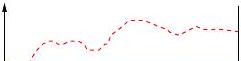
\includegraphics[max width=\textwidth]{2025_05_12_520db7cd238ba7b44f0fg-17(3)}
 & $\square$ & $\square$ & $\square$ &  \\
\hline
$\square$ &  &  &  &  \\
\hline
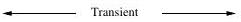
\includegraphics[max width=\textwidth]{2025_05_12_520db7cd238ba7b44f0fg-17(1)}
 & \multicolumn{4}{|c|}{Time} \\
\hline
\end{tabular}
\end{center}

b. Non-terminating simulation, fixed forcing "load", measures reported once or more in the steady state\\
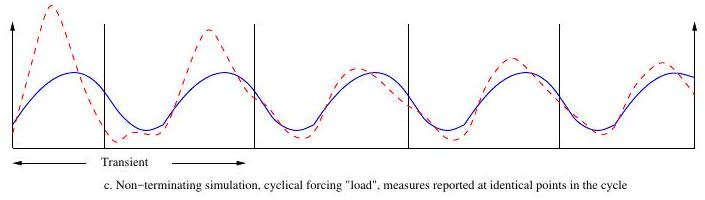
\includegraphics[max width=\textwidth, center]{2025_05_12_520db7cd238ba7b44f0fg-17(2)}

\section*{Output analysis of steady-state equilibrium}
\begin{itemize}
  \item We focus on non-terminating simulations.
  \item Assume we are using simulation to estimate some steady-state (i.e., "long run") performance measure, e.g. mean population, mean response time, resource utilisation, etc.
  \item The initial state is typically fixed (e.g. all queues empty), so the initial state probability distribution is different to the distribution after some time $t \gg 0$, say, and measures take time to settle.
  \item To avoid initialisation bias we must either\\
(1) Discard the initialisation transient by resetting the measures after some "warm-up" time has elapsed\\
(2) Measure for "long enough" to render any bias insignificant
\end{itemize}

\section*{Confidence intervals}
\begin{itemize}
  \item Discrete-event simulations are stochastic, so all outputs are random variables and each an observation of some measure, $\theta$, of interest.
  \item If $X_{i}, 1 \leq i \leq n, n \geq 1$ are steady-state observations from a simulation then an estimator for $\theta$ is the sample mean
\end{itemize}

$$
\bar{X}=\frac{1}{n} \sum_{i=1}^{n} X_{i}
$$

\begin{itemize}
  \item How can we quantify the uncertainty of the $\bar{X}$ estimate?
  \item Helpful to decide when to stop the simulation!
\end{itemize}

\section*{Confidence Interval for Mean}
\begin{itemize}
  \item We know by the CLT that $\bar{X} \sim N\left(\mu, \sigma^{2} / n\right)$.
  \item Then, if we knew $\sigma^{2}$, then for large $n$, since by the CLT
\end{itemize}

$$
P\left(-1.96 \leq \frac{\bar{X}-\mu}{\sigma / \sqrt{n}} \leq 1.96\right)=0.95
$$

\begin{itemize}
  \item In hypothesis testing, we condition on $H_{0}: \mu=\mu_{0}$ and study $\bar{X}$ with the last formula. But in simulation we do not know $\mu_{0}$ !
  \item However, CLT implies that we could generate many intervals
\end{itemize}

$$
\left[\bar{X}-1.96 \frac{\sigma}{\sqrt{n}}, \bar{X}+1.96 \frac{\sigma}{\sqrt{n}}\right]
$$

using different simulations and conclude that with 95\% probability we would have observed $\mu$ falling in the intervals.

\begin{itemize}
  \item This is known as the $\mathbf{9 5 \%}$ confidence interval for $\mu$.
\end{itemize}

\section*{Confidence Interval for Mean}
\begin{itemize}
  \item For $95 \%$ confidence interval for $\mu$ solve (two-sided estimate)
\end{itemize}

$$
0.975=\Phi\left(\frac{\bar{X}-\mu}{\sigma / \sqrt{n}}\right) \text { to }\left[\bar{X}-1.96 \frac{\sigma}{\sqrt{n}}, \bar{X}+1.96 \frac{\sigma}{\sqrt{n}}\right] .
$$

\begin{itemize}
  \item More generally, for any desired coverage probability level $1-\alpha$ we can define the $100(1-\alpha) \%$ confidence interval for $\mu$ by
\end{itemize}

$$
\left[\bar{X}-z_{1-\frac{\alpha}{2}} \frac{\sigma}{\sqrt{n}}, \bar{X}+z_{1-\frac{\alpha}{2}} \frac{\sigma}{\sqrt{n}}\right]
$$

where $z_{\alpha}$ is the $\alpha$-quantile of the standard normal (e.g., for $95 \%$ conf. int. we use $\alpha=0.05$ and hence $z_{0.975}$ )

\begin{itemize}
  \item Interpretation: Amongst all the possible intervals
\end{itemize}

$$
\bar{X} \pm z_{1-\frac{\alpha}{2}} \frac{\sigma}{\sqrt{n}}
$$

we might have observed $\alpha \%$ would have contained the unknown true parameter value $\mu$.

\section*{Example: $50 \%$ confidence intervals $(\alpha=0.5)$}
\begin{center}
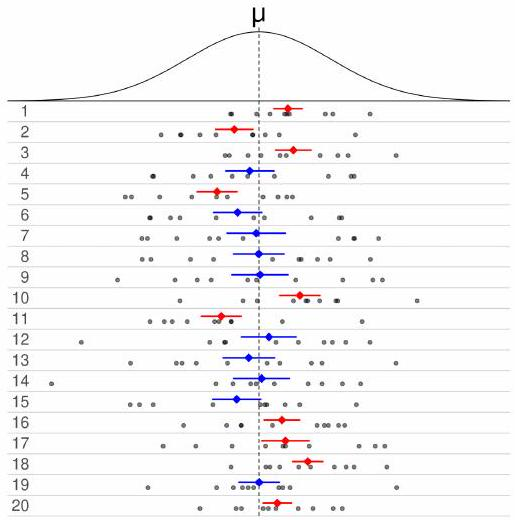
\includegraphics[max width=\textwidth]{2025_05_12_520db7cd238ba7b44f0fg-22}
\end{center}

The blue conf. int. contain the true mean, the red do not.\\
Image source: Wikipedia

\section*{Faulty reasoning on confidence intervals}
Wrong assertion: "I collected nobservations and created a 95\% confidence interval for $\mu$. The probability that the true mean is contained in the confidence interval I created is 0.95 ".

Correct assertion: "I collected nobservations and created a 95\% confidence interval for $\mu$. This particular interval may or may not contain $\mu$. However, if I were to create many confidence intervals like this one many times over, then approximately $95 \%$ of these intervals would cover the true mean $\mu$."

\section*{Dealing with unknown variance}
\begin{itemize}
  \item As we measure a population (simulated or real), we may not know the true variance $\sigma^{2}$, but only the (bias-corrected) sample variance $S^{2}$.
  \item How do the formulas change in this case? We proceed similarly to what we have seen for hypothesis testing.
  \item If $n>1$, a $100 \alpha \%$ confidence interval estimate for $\theta$ is
\end{itemize}

$$
\bar{X} \pm t_{n-1,1-\frac{\alpha}{2}} \frac{S}{\sqrt{n}}
$$

where $t_{\nu, p}$ is the $p$-quantile of the Student's $t$ distribution with $\nu$ degrees of freedom.

\section*{Confidence intervals in simulation}
\begin{itemize}
  \item How do we apply confidence intervals to simulation outputs?
  \item Looking at a single simulation run, a wider confidence interval suggests more uncertainty, while a narrower confidence interval suggests more precise estimation. This can help us decide if we should stop the simulation or not.
  \item Running $n$ independent replications, possibly in parallel, guarantees independence of the $X_{i}$
\end{itemize}

\section*{Confidence intervals in simulation}
\begin{itemize}
  \item Another approach is to run the model once, wait for it to warm up and reach (approximate) equilibrium, then divide the measurement time into batches, with $X_{i}$ coming from batch $i$\\
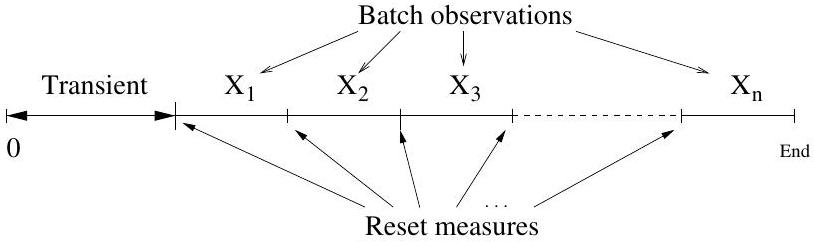
\includegraphics[max width=\textwidth, center]{2025_05_12_520db7cd238ba7b44f0fg-26}
  \item If each $X_{i}$ is the sample mean of batch $i$, this is called the batch means method
  \item Yet the $X_{i}$ may not be independent because the state at the end of one batch is the same as that at the start of the next!
  \item If the $X_{i}$ are dependent then we have to take covariances into account to build an exact confidence interval
  \item If the $X_{i}$ are dependent, then $\operatorname{Var}(\bar{X}) \neq \sigma^{2} / n$. Instead, it can be shown that
\end{itemize}

$$
\operatorname{Var}(\bar{X})=\frac{\sigma^{2}}{n}+\frac{1}{n^{2}}\left[2 \sum_{i=1}^{n-1} \sum_{j=i+1}^{n} \operatorname{Cov}\left(X_{i}, X_{j}\right)\right]
$$

\begin{itemize}
  \item If covariances are positive $S^{2} / n$ becomes an under-estimate of $\operatorname{Var}(\bar{X})$ and the computed confidence intervals are narrower than they should be
\end{itemize}

\section*{Example: A Simulation Model of a Server}
\begin{itemize}
  \item Here are three example time series plots for the mean wating time (moving average) from a simulation of a server system when the inter-arrival times are exponential with rate $\lambda=0.15$ :\\
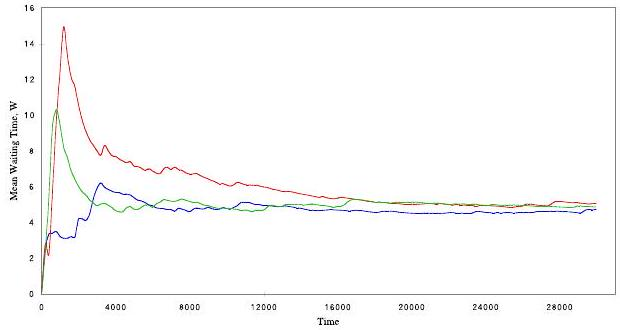
\includegraphics[max width=\textwidth, center]{2025_05_12_520db7cd238ba7b44f0fg-28}
  \item It looks as if the system is approaching equilibrium after around 15000 time units
  \item Now we increase the load to $\lambda=0.4 \ldots$\\
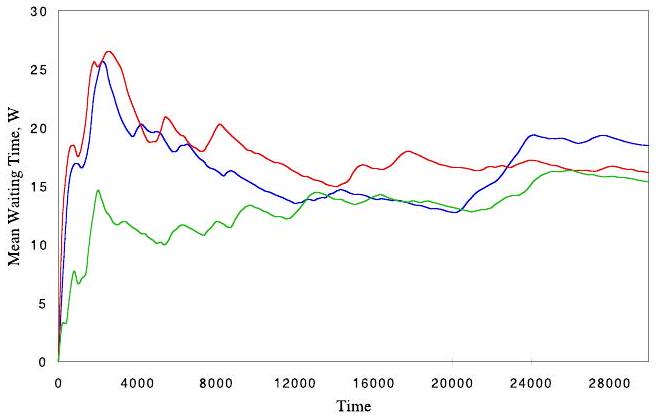
\includegraphics[max width=\textwidth, center]{2025_05_12_520db7cd238ba7b44f0fg-29}
  \item As $\lambda$ increases the system takes longer to reach equilibrium
  \item An an example, we would expect measurements taken between 15000 and 30000 time units, say, to have wider confidence intervals for $\lambda=0.4$ than for $\lambda=0.15$. Let's see...
\end{itemize}

\begin{center}
\begin{tabular}{c||c|c|c}
$\lambda$ & $W$ (exact) & Estimate & \begin{tabular}{c}
$90 \%$ Confidence Interval \\
$(10$ independent replications $)$ \\
\end{tabular} \\
\hline
0.10 & 4.86 & 4.839 & $(4.776,4.902)$ \\
0.15 & 5.42 & 5.267 & $(5.044,5.490)$ \\
0.20 & 6.16 & 6.198 & $(5.790,6.607)$ \\
0.25 & 7.17 & 6.679 & $(6.158,7.199)$ \\
0.30 & 8.68 & 8.662 & $(7.784,9.541)$ \\
0.35 & 11.25 & 11.726 & $(10.767,12.685)$ \\
0.40 & 16.86 & 16.295 & $(12.297,20.293)$ \\
0.45 & 42.45 & 30.765 & $(18.621,42.909)$ \\
\end{tabular}
\end{center}

The increasing widths of the confidence intervals is explain by the increased number of reachable states for the system, which results in increased variance in the measurements.

\section*{Example: State Space Coverage}
\begin{center}
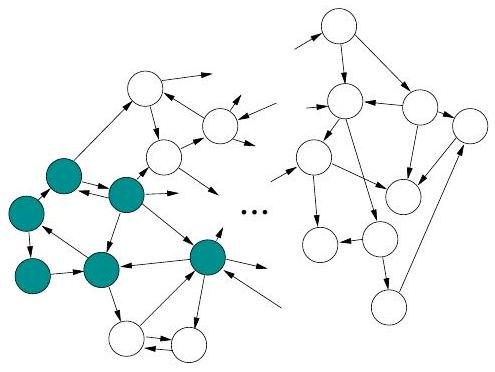
\includegraphics[max width=\textwidth]{2025_05_12_520db7cd238ba7b44f0fg-31(1)}
\end{center}

Parameterisation 1: Simulation time spent in a small number of states\\
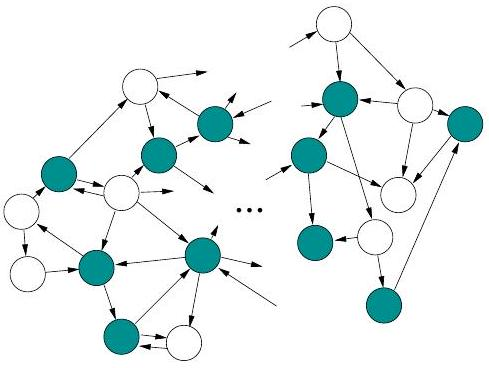
\includegraphics[max width=\textwidth, center]{2025_05_12_520db7cd238ba7b44f0fg-31}

Parameterisation 2: Simulation time spent covering a large number of states

For the same $T$, the confidence interval for the left model (low $\lambda$ ) tend to be narrower than the right (high $\lambda$ ).

Filled states: largest subset $S^{\prime} \subseteq S$ s.t. $\inf \left\{p_{i} \mid i \in S^{\prime}\right\} \geq \sup \left\{p_{j} \mid j \in S-S^{\prime}\right\}$ and $\sum_{i \in S^{\prime}} p_{i} \leq p_{\text {max }}$ for some $p_{\text {max }}$

\section*{Further remarks on confidence intervals}
\begin{itemize}
  \item Confidence intervals are seldom exact, one such case is if we sample $n$ i.i.d. $N\left(\mu, \sigma^{2}\right)$ random variables, since in this case $\bar{X}$ is always normally distributed.
  \item In practice, a computed confidence interval is typically approximate because of one or more of the following:
  \item $n$ is small and the $X_{i}$ are not normally distributed
  \item $n$ is "large" but not large enough
  \item The $X_{i}$ are not independent
  \item The true parameter is not restricted to be a mean. Confidence intervals also apply to arbitrary statistics $T(X)$ as uncertainty measures for estimates.
\end{itemize}

\section*{Distribution sampling}
\section*{The sampling problem}
\begin{itemize}
  \item Simulation depends on the ability to sample various discrete \& continuous random distributions, e.g. Uniform, Poisson, Exponential, Lognormal, Pareto, ...
  \item For r.v. $X$ with support $\operatorname{supp}(X)$, the objective is to define a sampling function:
\end{itemize}

$$
U(0,1) \rightarrow \operatorname{supp}(X)
$$

in terms of X's density/cdf (or pmf/cdf) function

\begin{itemize}
  \item We look at four commonly-used general methods:\\
(1) Inverse transform method\\
(2) Acceptance-Rejection (AR) method\\
(3) Convolution method\\
(9) Composition method
\end{itemize}

\section*{1. The Inverse Transform method}
\begin{itemize}
  \item Suppose $X$ is a continuous r.v. with cdf $F(x)=P(X \leq x)$ and that we are trying to sample $X$\\
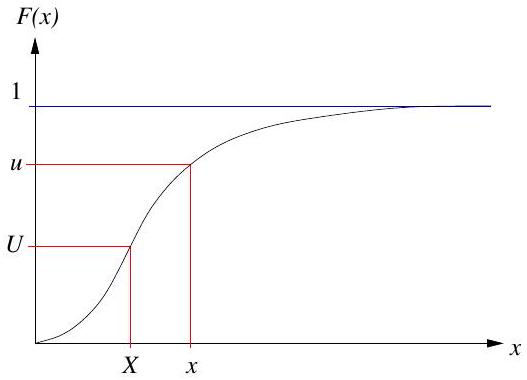
\includegraphics[max width=\textwidth, center]{2025_05_12_520db7cd238ba7b44f0fg-35}
  \item The inverse transform method iteratively samples a uniform distribution in $[0,1]$ and returns the corresponding quantile.
  \item In the figure, if $u \sim U(0,1)$ and $U \sim U(0,1)$, then we return as samples the $U$-quantile $(X)$ and the $u$-quantile $(x)$.
\end{itemize}

\section*{Example: Sampling an exponential}
\begin{itemize}
  \item If $X \sim \exp (\lambda)$ then
\end{itemize}

$$
F(x)=1-e^{-\lambda x}, \quad x \geq 0
$$

\begin{itemize}
  \item Setting $U=F(X)$ and inverting, we get:
\end{itemize}

$$
\begin{aligned}
U & =1-e^{-\lambda X} \\
1-U & =e^{-\lambda X} \\
\log (1-U) & =-\lambda X \\
\frac{-\log (1-U)}{\lambda} & =X
\end{aligned}
$$

\begin{itemize}
  \item So, if $U \sim U(0,1)$, then $-\log (1-U) / \lambda \sim \exp (\lambda)$
  \item Note that we can replace $1-U$ with $U$ since $(1-U) \sim U(0,1)$, namely $-\log (U) / \lambda$
\end{itemize}

\section*{Sampling discrete (empirical) distributions}
\begin{itemize}
  \item We can use the inverse transform method also to sample a discrete r.v., $X$ by inverting its cumulative distribution function, $F_{X}(x)$ (a "step function"), e.g.\\
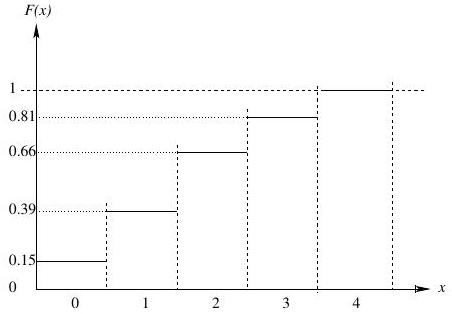
\includegraphics[max width=\textwidth, center]{2025_05_12_520db7cd238ba7b44f0fg-37}
\end{itemize}

\begin{center}
\begin{tabular}{|c|cc|}
\hline
$x$ & $p(X=x)$ & $F(x)$ \\
\hline
0 & 0.15 & 0.15 \\
1 & 0.24 & 0.39 \\
2 & 0.22 & 0.61 \\
3 & 0.20 & 0.81 \\
4 & 0.19 & 1.00 \\
\hline
\end{tabular}
\end{center}

\begin{itemize}
  \item If $U \sim U(0,1)$, then the inverse transform methods returns
\end{itemize}

$$
X=\min \{x: F(x) \geq U\}
$$

\section*{2. The Acceptance-Rejection (AR) Method}
\begin{itemize}
  \item If $F(x)$ cannot be explicitly inverted (e.g., normal cdf) we can sometimes work with the corresponding density function $f(x)$
  \item We choose a density function $g(x)$ easy to sample from
  \item Now we try to find a constant, $c$, so that $c g(x)=h(x)$ dominates $f(x)$ for all $x$ :\\
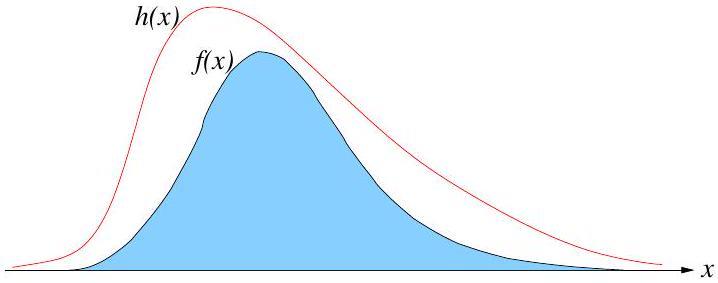
\includegraphics[max width=\textwidth, center]{2025_05_12_520db7cd238ba7b44f0fg-38}
  \item By construction, $c$ is the area under $h(x)$ :
\end{itemize}

$$
c=c \int_{x} g(x) d x=\int_{x} h(x) d x
$$

\begin{itemize}
  \item AR Algorithm:\\
(1) Let $X$ be a sample from the r.v. whose density function is $g(x)$\\
(2) Generate a $U(0,1)$ sample, $U$, and let $Y=U h(X)$\\
(3) If $Y \leq f(X)$, i.e. if $U \leq \frac{f(X)}{h(X)}=\frac{f(X)}{c g(X)}$, then accept $X$; otherwise reject it and start again
  \item It's a "dart throwing" exercise (Monte Carlo simulation)
  \item By construction, the samples $X$ and $Y$ define a point that lies under $h(X)$; if ( $X, Y$ ) lies under $f(X)$ as well we accept $X$\\
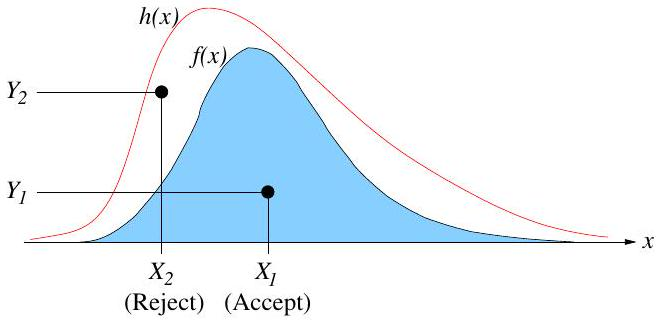
\includegraphics[max width=\textwidth, center]{2025_05_12_520db7cd238ba7b44f0fg-39}
\end{itemize}

\section*{Example: Half-normal}
\begin{itemize}
  \item Suppose we wish to sample a standard "half-normal" distribution:
\end{itemize}

$$
f(x)=\frac{2}{\sqrt{2 \pi}} e^{-x^{2} / 2}, \quad x \geq 0
$$

\begin{itemize}
  \item We arbitrarily choose $g(x)=e^{-x}$ (exponential, parameter 1 ), as it is easy to sample
  \item We need an $h(x)=c g(x)$ that dominates $f(x)$ for $x \geq 0$
  \item $c$ can be found by computing $\max _{x} f(x) / g(x)$, i.e.
\end{itemize}

$$
c=\max _{x \geq 0} \frac{\frac{2}{\sqrt{2 \pi}} e^{-x^{2} / 2}}{e^{-x}}=\max _{x \geq 0} \sqrt{\frac{2}{\pi}} e^{x-x^{2} / 2}
$$

\begin{itemize}
  \item By differentiation, this is maximal when $x=1$, thus\\
$c=\sqrt{2 / \pi} e^{1 / 2}=\sqrt{2 e / \pi}$, so
\end{itemize}

$$
h(x)=\sqrt{2 e / \pi} e^{-x} \text { and } \frac{f(x)}{h(x)}=e^{-(x-1)^{2} / 2}
$$

\begin{center}
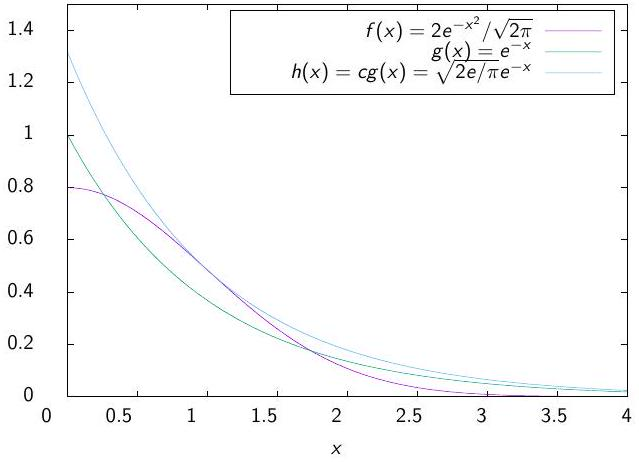
\includegraphics[max width=\textwidth]{2025_05_12_520db7cd238ba7b44f0fg-41}
\end{center}

\begin{itemize}
  \item Notice that $h(x)$ dominates $f(x)$
  \item Thus, sample $X$ from $-\log \left(1-U_{1}\right)$ (inverse transform method applied to exponential distribution, parameter 1) and accept $X$ iff $U_{2} \leq \frac{f(X)}{h(X)}=e^{-(X-1)^{2} / 2}$, where $U_{1}, U_{2} \sim U(0,1)$
  \item The efficiency depends on the number of rejections $R$ before accepting a value of $X$
  \item The probability of accepting $X$, call it $p$, is simply the ratio of the areas of the two functions, i.e. $p=1 / c$
  \item Since each sample from $g(x)$ is independent, the number of iterations $/$ required before accepting it as a sample of $f(x)$ is geometrically distributed, i.e.:
\end{itemize}

$$
E(I)=\frac{1}{p}=c
$$

So the expected number of rejections is $R=c-1$.

\begin{itemize}
  \item Example: For the half-normal (above) $c=\sqrt{2 e / \pi}=1.315$; this equates to $2 \times 1.315=2.63$ random $U(0,1)$ samples on average per sample (very efficient!).
\end{itemize}

\section*{3. The Convolution Method}
\begin{itemize}
  \item Some random variables are defined as the sum of two or more independent random variables
  \item We can sample the individual distributions and sum the results
  \item Example: An Erlang $(k, \theta)$ random variable, $X$ say, is defined as the sum of $k$ independent exponentially-distributed random variables $X_{i}$, each with rate parameter $\theta$\\
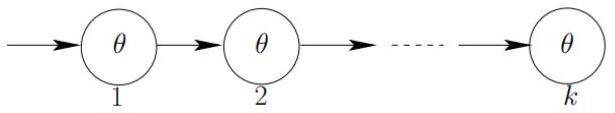
\includegraphics[max width=\textwidth, center]{2025_05_12_520db7cd238ba7b44f0fg-43}
  \item Notice that
\end{itemize}

$$
E[X]=E\left[X_{1}+\ldots+X_{k}\right]=\frac{1}{\theta}+\frac{1}{\theta}+\cdots+\frac{1}{\theta}=\frac{k}{\theta}
$$

\begin{itemize}
  \item We can generate Erlang $(k, \theta)$ samples using the sampler for the exponential distribution: if $X_{i} \sim \exp (\theta)$ then
\end{itemize}

$$
X=\sum_{i=1}^{k} X_{i} \sim \operatorname{Erlang}(k, \theta)
$$

\begin{itemize}
  \item If $U_{i} \sim U(0,1)$ then $X_{i}$ is sampled using $-\log U_{i} / \theta$
  \item We can save the more expensive log calculations in the summation by turning the sum into a product:
\end{itemize}

$$
X=\sum_{i=1}^{k}-\frac{\log U_{i}}{\theta}=-\frac{1}{\theta} \log \prod_{i=1}^{k} U_{i}
$$

\section*{4. The Composition Method}
\begin{itemize}
  \item Consider a discrete RV $Y$ with $\operatorname{supp}(Y)=\{1, \ldots, n\}$ and a continuous RV $X$ with conditional density $f_{i}(x) \equiv f(x \mid Y=i)$.
  \item An application of the Law of Total Probability gives
\end{itemize}

$$
f(x)=w_{1} f_{1}(x)+w_{2} f_{2}(x)+\ldots+w_{n} f_{n}(x)
$$

where $w_{i}=P(Y=i)$ and thus $\sum_{i=1}^{n} w_{i}=1$. This is called a mixture distribution.

\begin{itemize}
  \item The Composition Method is a sampler for mixtures:
  \item Pick $i$ with probability $w_{i}$ (discrete distribution sampling)
  \item Sample from the density $f_{i}(x)$
  \item This method applies similarly also to cdfs and pmfs.
\end{itemize}

\section*{Example: a Gaussian Mixture Model (GMM)}
A GMM with parameters $\left(\mu_{i}, \sigma_{i}^{2}\right), 1 \leq i \leq n$, has density

$$
f(x)=\sum_{i=1}^{n} w_{i} f_{i}(x), \quad f_{i}(x)=\frac{1}{\sqrt{2 \pi \sigma_{i}^{2}}} \exp \left(-\frac{\left(x-\mu_{i}\right)^{2}}{2 \sigma_{i}^{2}}\right)
$$

For equal $\sigma_{i}^{2}$, but different means $\mu_{i}$, we may get, e.g.:\\
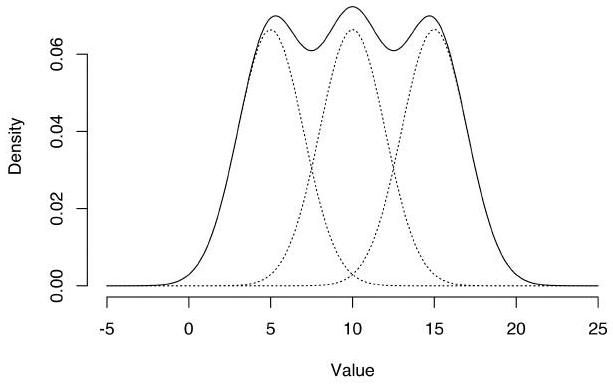
\includegraphics[max width=\textwidth, center]{2025_05_12_520db7cd238ba7b44f0fg-46}

The composition method samples from $f_{i}(x)$ with probability $w_{i}$.


\end{document}